\section{Science Validation} \label{sect:scival}

\subsection{Definition}

We define DM Science Validation as the process by which we
assess the as-built Data Management system meets the needs of the
scientific community and other identified stakeholders.

We assess the projected and realized scientific usability of the system by
periodically exercising the integrated system in a way that goes beyond
synthetic unit and integration tests and verification of piece-wise
requirements as described in previous sections.  In other words, we \emph{
attempt to use the system in ways we expect it to be used by the ultimate
users of the system, scientists}.  An example may be performing a mock
science study on the results of processing of precursor data, or performing
a mock science-like activity (e.g., interactive analysis of time-domain
datasets) on a partially stood-up service (e.g., the Notebook aspect of the
LSST Science Platform).  We record and analyze any issues encountered in
such usage, and feed this information back to the DM Science and DM
development teams.

Science Validation exercises are designed to close the design-build-verify
loop, and enable one to measure the degree to which the requirements,
designs, the as-built system, and future development plans continue to
satisfy stakeholder needs.  They also provide valuable feedback about
modifications needed to ensure the delivery of a scientifically capable
system.  Ultimately, SV activities transfer into commissioning SV activities
and provide training to the future members of the Commissioning team.

% While this Section describes the high-level goals, scope, and organization
% of the Science Verification effort, more details are provided in
% Document-XXX.

\subsection{Schedule and Execution}

\subsubsection{Schedule}

Unlike the verification and rehearsal activities, which correspond to high
level milestones, validation activities are planned and prepared in a rolling
wave fashion in parallel with development activities (on a 6-month cycle, or
perhaps a year). The SV activities will typically be designed so as to
exercise the capabilities of the system expected to be delivered at the end of
a given development cycle.  The Science Validation (SV) team guides the
definition of goals of those activities, in close consultation with the DM
Project Manager.


By their nature, SV activities will typically lag behind
deliveries of the (sub)system being verified -- ideally, they will commence
immediately upon delivery. Preparatory SV activities (e.g., identification and
acquisition of suitable datasets, identification of potential Science
Collaboration resources to include on the activity, or development of
activity-specific analysis codes) will commence as early as feasible. DM SV
Scientist will coordinate the execution of all SV activities.

SV activities should aim to take no longer than two months to conclude, to
enable rapid actionable feedback to DM Management and DM Subsystem Science.

\subsubsection{Execution}

Science Validation activities typically follow the successful execution of
unit and integration test activities described in the previous sections,
especially the larger ``dress rehearsals'' and ``data challenges'' as
listed in Section~\ref{sect:schedule} (Master Schedule).

Following successful service stand-up or data challenge execution (at
integration and unit test level), the generated data products or integrated
services are turned over to the SV team.  The SV team performs additional
tests and data analyses to exercise the integrated system and assess its
quality relative to expectations for the current phase of construction.
This assessment is fed back to DM Subsystem Science and Systems Engineering
teams to inform them about the status and needed improvements to the system.

Beyond reporting on the results, the SV team examines the tests or
procedures developed in this phase and identifies those that are good new
metrics of system quality and could be run in an automated fashion.  These
are fed back to the development teams for productizing and incorporation
into the automated QC systems.

\subsection{Deliverables}

Key deliverables of Science Validation activities are:
\begin{itemize}

\item Reports on the assessed capability of the Data Management System to
satisfy stakeholder needs.  The assessments shall take into account the
expected maturity of the system being tested.

\item Recommendations for improvements and changes, both in the quality of
as-constructed systems (i.e., what needs to be built differently or better,
to make it more consistent with the system vision), as well as the overall
system vision (i.e., recommendations on where the vision may need to be
modified to fully respond to stakeholder needs).

\item Measurements of performance metrics that do not lend themselves to
easy automation (e.g., science activities requiring human involvement, like
visual classification, or UX tests).

\item Identification of new performance metrics to be tracked, including
potential deliveries of code to the DM Construction and I\&T teams for
inclusion in automated quality control pipelines.

\item Other deliverables as charged when chartering a particular SV exercise.

\end{itemize}

\subsection{Organization and Resources}

\begin{figure}
\centering
\scalebox{0.5}{\hskip 0.0in \includegraphics[trim={2.4cm 3cm 2.4cm
3cm},clip,page=2]{figures/dm-subsystem-science.pdf}}
\caption{Organogram of the Data Management Science Validation Team.
The group is chaired by the DM Science Validation Scientist,
with the DM Science Pipelines Scientist and Institutional Science Leads making up
the permanent membership. Depending on the SV activities being executed at any
given time, the group may draw on additional temporary members from DM SST Staff,
the broader DM Construction staff, as well as external scientists (e.g.,
Science Collaboration members committed to assisting SV goals). SV membership
is reassessed on a cycle by cycle basis, with estimates incorporated in the
long-term plan.
\label{fig:DMsvg}}
\end{figure}

The DM Subsystem Scientist is accountable to the LSST Project Scientist for
successful execution of DM Science Validation activities.  This
responsibility is delegated to the \textbf{DM Science Validation Scientist},
who leads the Science Validation (SV) team.

The SV team guides the definition of goals and receives the products of
dress rehearsal activities, consistent with the long-term testing roadmap
defined in Section~\ref{sect:schedule}.  Decisions on strategic goals of SV exercises are made
in close consultation and coordination with the DM Project Manager and
Subsystem Scientist.  The results of SV activities are reported to the DM
Project Manager and Subsystem Scientist.

SV activities draw on resources of the DM System Science Team, but may also
tap into the broader construction team if needed (and as jointly agreed upon
with the DM Project Manager), as well as contributors from the LSST Science
Collaborations.  Additional members may added as needed, depending on SV
activities being considered and based on the recommendation of the DM SV
Scientist and resource constraints.

The SV Scientist, the DM Science Pipelines Scientist, and all Institutional
Science Leads are ex-officio members of the SV Team.  DM Project Scientist and
Managers are not formal members, but monitor the work of the group.

\subsubsection{Example}

An example of a Science Validation activity may be as follows:

\begin{itemize}

\item Based on the long-term development roadmap and new capabilities
expected to be delivered, the at the beginning of a 6-month cycle the SV
Team defines the goals of a data challenge to be executed at the end of the
cycle.  For the purposes of this example, we assume a major new feature to
be delivered is astrometric calibration and estimation of proper motions.

\item A small data release production using HSC data is defined that
should result in a data set sufficient to measure the size and orientation
of velocity ellipsoids in the Galactic halo.  If such measurement are a
success, they would independently validate the newly added global
astrometric calibration and proper motion measurement capability.

\item At the end the development cycle, the Science Pipelines team delivers to the
proto-Operations team a documented and internally tested set of DRP
pipelines with the new capabilities as defined above.  The pipelines pass
all unit and small-scale integration tests.  The proto-Operations team
deploys and re-verifies the received pipelines in the I\&T environment
designed to closely mimic the production environment.  They verify that the
pipeline integrates well with the orchestration system and is capable of
executing medium-to-large scale processing.  The pipelines pass integration
tests.

\item The data challenge is operationally planned and executed by the
proto-Operations team, including the execution of any predefined QA metrics.
The data products and test results are turned over to the Science
Validation team.

\item The Science Validation team performs the analysis needed to achieve
SV exercise goals (the measurement of velocity ellipsoids, in this case).

\item The results and conclusions derived from the data challenge are fed back to
the DRP team, DM Project Management, and DM Subsystem Science; they may be
used to assess the overall quality of the product, pass a formal
requirement, and/or inform future construction decisions.

\item Any newly developed but broadly useful tests are identified as such,
and fed to the I\&T team for inclusion into the battery of tests that are
run on a regular basis.

\end{itemize}
